\documentclass[thesis]{subfiles}

\begin{document}
%*******************************************************************************
%*********************************** Future Work *****************************
%*******************************************************************************

\chapter{Future Work}  %Title of the First Chapter
\label{futurework}

%********************************** %First Section  **************************************

Here we outline the research directions I plan to pursue, planned conference submissions and a preliminary research schedule.

\section{Future Research Topics}

\subsection{Learning a Basis for Spatial and Channel Extents of Filters}
\label{journalplan}
The work of chapters \ref{lowrankfilters} and \ref{deeproots} explore learning more efficiently by reducing the learned parameters in the spatial and channel extents, respectively, of convolutional filters. These naturally lend themselves to being merged into a single effective method for training with low-rank basis filters. We plan to submit a journal article in which both methods are merged and explored in new results on state-of-the-art deep networks.

\subsection{Random Low-Dimensional Projection in Deep Neural Network Optimization}
\label{pairablation}
Here we present the initial findings from on-going research investigating neural co-dependence in neural networks. The results presented for a CIFAR VGG network trained with dropout and our dropproject methods motivated further research into the salient action behind the increased generalization of networks using dropout. The first step is to reproduce these results on a state-of-the-art network for ImageNet, and I am currently running experiments on AlexNet and Inception v3, which both extensively use dropout.

Assuming that further experiments confirm the findings, I plan to investigate more principled methods of random projection in deep neural networks, as a method to aid optimization and improve training time.% Given our insight into Dropout, the Johson-Lindenstrauss lemma gives us bounds on the minimum number of dimensions in which pairwise distances are preserved in random projection to a given maximum pairwise error $\epsilon$. This is equivalent to giving bounds on the appropriate dropout ratio for a given training set size.


\subsubsection{Adverse Neural Co-adaption}
\citet{Hinton2012} proposed dropout as a regularization method for neural networks. In randomly dropping out hidden units -- zeroing out a random subset on each layer -- it was claimed that complex co-adaptions of these hidden units on training data, which do not generalize to the test set, are prevented. In practice dropout has seen remarkable success in improving the generalization of large neural networks, especially in the context of large fully-connected layers. Several follow-up methods have similarly suggested alternative methods of preventing this co-adaption\mynote{TODO: cite}.

Although empirically dropout works well, the claim that hidden units learn to co-adapt has not itself been well demonstrated, and seemingly straightforward methods of doing have serious drawbacks. Showing the covariance/correlation between pairs of hidden units doesn't give the full story, since covariance shows the linear relationship between the units, but in a deep network this relationship is likely to be highly non-linear. Mutual information cannot be used either since most modern networks need to use unbounded activation functions, such as ReLUs, in order to train effectively.

A crude but effective method of analyzing the importance of hidden units in neural networks is ablation -- zeroing out certain units in a trained network of interest, and observing the effect on the training and test loss. This method can be extended to empirically evaluate the importance of pairs of hidden units in trained neural networks. For each pair of hidden units, zero out the parameters of both units, and observe the effect on the loss calculated over the training/test set: pairwise ablation. This is however very expensive since each pair of hidden units must be evaluated over the entire dataset. 

\begin{figure}[tp]
	\centering
	\begin{subfigure}[b]{0.45\textwidth}
		\begin{tikzpicture}
		\begin{axis}[
		width=\textwidth,
		axis equal image,
		%    axis lines=none,
		enlargelimits=false,
		%colorbar,
		%colorbar style={
		%    yticklabel={\pgfmathprintnumber\tick\,\%},
		%    yticklabel style={font=\footnotesize}
		%},
		%    colormap name={Paired-12},
		colormap name={RdYlBu-9},
		baseline,
		scale only axis,
		xmax = 64,
		xmin = 0,
		ymax = 64,
		ymin = 0,
		]
		%\addplot[surf,
		%    view={0}{90},
		\addplot [
		matrix plot*,
		point meta=explicit,
		point meta min=-1.6E-02,
		point meta max=1.0E-02,
		] file [
		x index=0,
		y index=1,
		meta index=2,
		]{ablationdata/resnet50/ablation_train_top5_conv1_square.dat};
		\end{axis}
		\end{tikzpicture}
		\caption{Top-5 training acc.~diff.~for filter pairs}
		\label{fig:resnet50ablation_conv1_top5_train_hist}
	\end{subfigure}~
	\begin{subfigure}[b]{0.45\textwidth}
		\begin{tikzpicture}
		\begin{axis}[
		width=\textwidth,
		axis equal image,
		%    axis lines=none,
		enlargelimits=false,
		colorbar,
		colorbar style={
			yticklabel={\pgfmathprintnumber\tick\,\%},
			yticklabel style={font=\footnotesize}
		},
		colormap name={RdYlBu-9},
		baseline,
		scale only axis,
		xmax = 64,
		xmin = 0,
		ymax = 64,
		ymin = 0,
		]
		%\addplot[surf,
		%    view={0}{90},
		\addplot [
		matrix plot*,
		point meta=explicit,
		point meta min=-1.6E-02,
		point meta max=1.0E-02,
		] file [
		x index=0,
		y index=1,
		meta index=2,
		]{ablationdata/resnet50/ablation_test_top5_conv1_square.dat};
		\end{axis}
		\end{tikzpicture}
		\caption{Top-5 validation acc.~diff.~for filter pairs}
		\label{fig:resnet50ablation_conv1_top5_test_hist}
	\end{subfigure}\\
	
	\begin{subfigure}[b]{0.45\textwidth}
		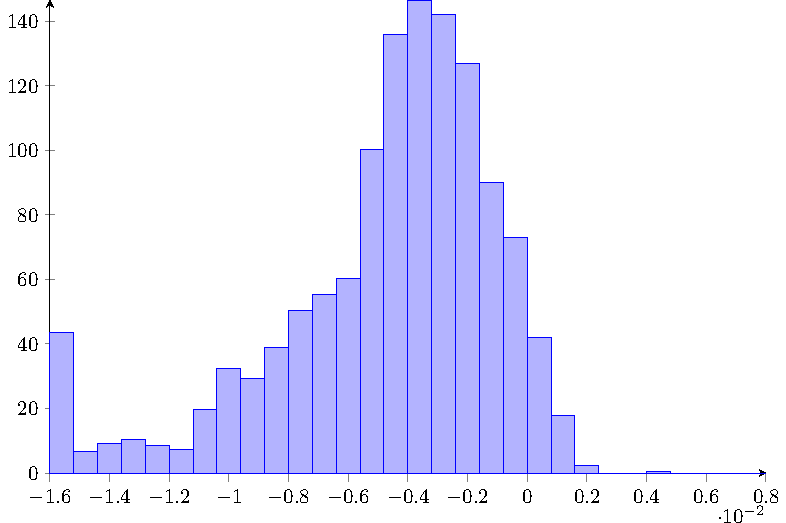
\includegraphics[width=\textwidth]{resnet50histtrain}
		\caption{Histogram of change in top-5 training acc.}
		\label{fig:resnet50ablation_conv1_top5_train}
	\end{subfigure}
	~
	\begin{subfigure}[b]{0.45\textwidth}
		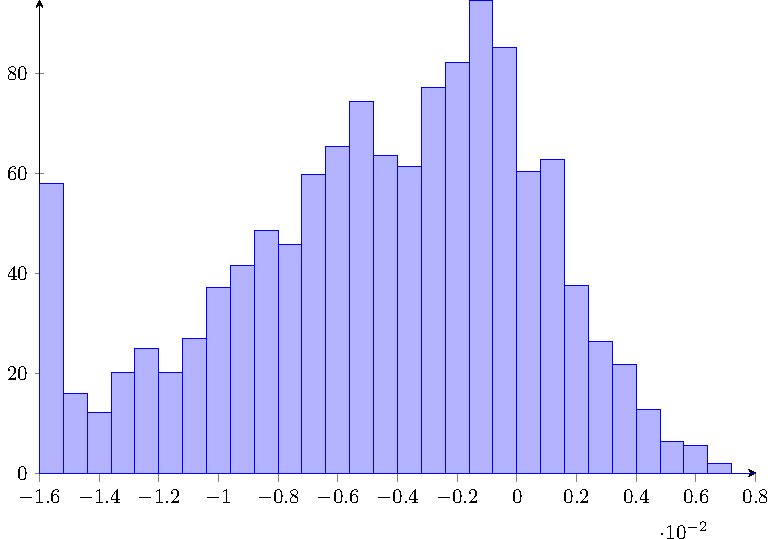
\includegraphics[width=\textwidth]{resnet50histtest}
		\caption{Histogram of change in top-5 val.~acc.}
		\label{fig:resnet50ablation_conv1_top5_test}
	\end{subfigure}
	
	%\input{resnet50fig.tex}
	\caption[Pairwise filter ablations in ResNet 50]{Histogram of the change in top-5 accuracy for all pairwise filter ablations of a 2500 randomly sampled images from the ILSVRC training/validation set in \texttt{conv1} of ResNet-50.}
	\label{fig:resnet50ablation_conv1_top5}
\end{figure}
Figure \ref{fig:resnet50ablation_conv1_top5} shows the results of pairwise ablation on the first convolutional layer (conv1) of a Resnet-50~\citet{He2015} network trained on ILSVRC2012~\citep{ILSVRC2015}. This is evaluated on random subsets (5000 images) of both the training set (Fig.~\ref{fig:resnet50ablation_conv1_top5_train},\ref{fig:resnet50ablation_conv1_top5_train_hist}) and validation set (Fig.~\ref{fig:resnet50ablation_conv1_top5_test},\ref{fig:resnet50ablation_conv1_top5_test_hist}).

While, as expected, most pairwise ablations result in a decrease in accuracy, a small but significant number of pairwise ablations result in an \emph{increase} in accuracy (and decrease in loss). For the validation set this seems to provide clear evidence of hidden units co-adapting, and hence over-fitting to the training data. Surprisingly however, this effect is also evident when evaluating on the training set, and by definition cannot be explained by over-fitting. We observed similar effects on all other layers of the network (see supplemental).

We claim that the observed neural co-adaption is in fact a symptom of the problem of pathological surface curvature, which first-order optimization cannot fully address. This curvature is described by the Hessian, and for each pair of hidden units, the mixed partial second order derivatives. For two hidden units in a network with parameters $w_1, w_2, \ldots, w_N$ and with loss function $L(w_1, w_2, \ldots, w_N)$, and hidden units $w_i$ and $w_j$, where $i,j \in [1, N]$ are related to the loss with the mixed partial second order derivatives,

\begin{equation}
\frac{\partial^2 L}{\partial w_i \partial w_j}, \frac{\partial^2 L}{\partial w_j \partial w_i}.
\end{equation}

When training with a second-order optimizer, these pairwise derivatives are used along with the diagonal second order derivatives (\ie $\frac{\partial^2 L}{\partial w_i^2}$) , whereas when training with gradient descent, only the first order derivatives (\ie $\frac{\partial L}{\partial w_i}$) are used. However, the effect is more than pairwise, and hence higher order mixed partials would be required to prevent any form of co-adaption.

Dropout does reduce the observed adverse co-adaption on a layer, which is surprising if dropout is in fact only a method of regularization.

\subsubsection{Dropout as Random Low-dimensional Projection}
Dropout can also be thought of as a orthogonal projection of the error surface onto a random lower-dimensional subspace, in which the curvature of the error surface may no longer exhibit pathological issues, and optimization may be easier. For example, if in a subset of the dimensions, a deep valley exists, and these dimensions are dropped-out. Random projection is a well established method for dimensionality reduction of high dimensional spaces~\citep{kaski1998dimensionality,fodor2002survey}.
If a layer has $N$ nodes, and a weight matrix $W$, and input vector $x$, then dropout on the layer of $K/N$ nodes may be defined as the transformation:

\begin{equation}
\textrm{Dropout}(\mathbf{W}) = \mathbf{D}_{i} \mathbf{W},
\end{equation}

where $D$ is a diagonal binary matrix, with rank $K$, defining an orthogonal projection onto a $K$-dimensional subspace. 

To demonstrate that it is this projection, rather than the zeroing out of neurons itself, that is responsible for performance improvements with dropout, we can instead perform a random projection in a different orthogonal co-ordinate basis, which does not dropout (zero) any neurons. To do this we can first rotate the parameters with random rotation matrix into a non-axis aligned co-ordinate basis, and perform dropout (orthogonal projection) in the rotated space, and then rotate back into the original co-ordinate basis:

\begin{equation}
\textrm{Dropproject}(\mathbf{W}_l) = \mathbf{R}^{-1}\textrm{Dropout}(\mathbf{R} \mathbf{W}_l),
\end{equation}

for a random rotation matrix $\mathbf{R}\in \textrm{SO}_N$. ``Dropproject'' avoids zeroing out any of the units, while still performing an equivalent projection as that in dropout.

\begin{figure}[tp]
	
	\begin{subfigure}[b]{\textwidth}
		\begin{tikzpicture}
		\begin{axis}[
		thick,
		cycle multi list={Set1-5},
		scale only axis,
		axis x line=bottom,
		axis y line=left,
		%axis line style={thick},
		width=\linewidth,
		height=0.2\linewidth,
		xlabel={Epochs},
		ylabel={Log Loss},
		ymode=log,
		legend columns=-1,
		legend style={at={(0.5,1.1)},anchor=south,text depth=.5ex},
		]
		
		\addplot +[mark=none] table [x=epoch, y expr=\thisrow{main/loss}, col sep=comma]{ablationdata/dropproject/train_standard.csv};
		\addplot +[mark=none] table [x=epoch, y expr=\thisrow{main/loss}, col sep=comma]{ablationdata/dropproject/train_dropout.csv};
		\addplot +[mark=none] table [x=epoch, y expr=\thisrow{main/loss}, col sep=comma]{ablationdata/dropproject/train_dropproject.csv};
		\addplot +[mark=none] table [x=epoch, y expr=\thisrow{main/loss}, col sep=comma]{ablationdata/dropproject/train_dropproject10.csv};
		\addplot +[mark=none] table [x=epoch, y expr=\thisrow{main/loss}, col sep=comma]{ablationdata/dropproject/train_dropprojectrandom.csv};
		
		\legend{
			Standard, 
			Dropout, 
			Dropproject,
			DP-Random 10,
			DP-Random}
		
		\end{axis}
		
		\end{tikzpicture}
		\caption{CIFAR Training Log Loss}
		\label{fig:cifar_dropproject_train_loss}
	\end{subfigure}
	
	\begin{subfigure}[b]{\textwidth}
		
		\begin{tikzpicture}
		\begin{axis}[
		thick,
		cycle multi list={Set1-9},
		scale only axis,
		axis x line=bottom,
		axis y line=left,
		%axis line style={thick},
		width=\linewidth,
		height=0.2\linewidth,
		xlabel={Epochs},
		ylabel={Log Loss},
		ymode=log,
		%    ymax=1,
		ymin=0,
		]
		
		\addplot +[mark=none] table [x=epoch, y expr=\thisrow{validation/main/loss}, col sep=comma]{ablationdata/dropproject/train_standard.csv};
		\addplot +[mark=none] table [x=epoch, y expr=\thisrow{validation/main/loss}, col sep=comma]{ablationdata/dropproject/train_dropout.csv};
		\addplot +[mark=none] table [x=epoch, y expr=\thisrow{validation/main/loss}, col sep=comma]{ablationdata/dropproject/train_dropproject.csv};
		\addplot +[mark=none] table [x=epoch, y expr=\thisrow{validation/main/loss}, col sep=comma]{ablationdata/dropproject/train_dropproject10.csv};
		\addplot +[mark=none] table [x=epoch, y expr=\thisrow{validation/main/loss}, col sep=comma]{ablationdata/dropproject/train_dropprojectrandom.csv};
		
		\end{axis}
		\end{tikzpicture}
		
		\caption{CIFAR Test Log Loss}
		\label{fig:cifar_dropproject_test_loss}
	\end{subfigure}
	
	\begin{subfigure}[b]{\textwidth}
		\begin{tikzpicture}
		\begin{axis}[
		thick,
		cycle multi list={Set1-9},
		scale only axis,
		axis x line=bottom,
		axis y line=left,
		%axis line style={thick},
		width=\linewidth,
		height=0.2\linewidth,
		xlabel={Epochs},
		ylabel={Training Error},
		%    ymax=1,
		%    ymin=0,
		]
		
		\addplot +[mark=none] table [x=epoch, y expr=1-\thisrow{main/accuracy}, col sep=comma]{ablationdata/dropproject/train_standard.csv};
		\addplot +[mark=none] table [x=epoch, y expr=1-\thisrow{main/accuracy}, col sep=comma]{ablationdata/dropproject/train_dropout.csv};
		\addplot +[mark=none] table [x=epoch, y expr=1-\thisrow{main/accuracy}, col sep=comma]{ablationdata/dropproject/train_dropproject.csv};
		\addplot +[mark=none] table [x=epoch, y expr=1-\thisrow{main/accuracy}, col sep=comma]{ablationdata/dropproject/train_dropproject10.csv};
		\addplot +[mark=none] table [x=epoch, y expr=1-\thisrow{main/accuracy}, col sep=comma]{ablationdata/dropproject/train_dropprojectrandom.csv};
		
		\end{axis}
		
		\end{tikzpicture}
		\caption{CIFAR Training Error}
		\label{fig:cifar_dropproject_train_acc}
	\end{subfigure}
	
	\begin{subfigure}[b]{\textwidth}
		
		\begin{tikzpicture}
		\begin{axis}[
		thick,
		cycle multi list={Set1-9},
		scale only axis,
		axis x line=bottom,
		axis y line=left,
		%axis line style={thick},
		width=\linewidth,
		height=0.2\linewidth,
		xlabel={Epochs},
		ylabel={Test Error},
		%    ymin = 0,
		]
		
		\addplot +[mark=none] table [x=epoch, y expr=1-\thisrow{validation/main/accuracy}, col sep=comma]{ablationdata/dropproject/train_standard.csv};
		\addplot +[mark=none] table [x=epoch, y expr=1-\thisrow{validation/main/accuracy}, col sep=comma]{ablationdata/dropproject/train_dropout.csv};
		\addplot +[mark=none] table [x=epoch, y expr=1-\thisrow{validation/main/accuracy}, col sep=comma]{ablationdata/dropproject/train_dropproject.csv};
		\addplot +[mark=none] table [x=epoch, y expr=1-\thisrow{validation/main/accuracy}, col sep=comma]{ablationdata/dropproject/train_dropproject10.csv};
		\addplot +[mark=none] table [x=epoch, y expr=1-\thisrow{validation/main/accuracy}, col sep=comma]{ablationdata/dropproject/train_dropprojectrandom.csv};
		
		\end{axis}
		\end{tikzpicture}
		
		\caption{CIFAR Test Error}
		\label{fig:cifar_dropproject_test_acc}
	\end{subfigure}
	
	\caption[Dropout \vs dropproject for VGG/CIFAR-10]{Training and test curves for a VGG network on CIFAR comparing dropout to dropproject.}
	\label{fig:cifar_dropproject}
\end{figure}

Fig.~\ref{fig:cifar_dropproject} compares the effect of dropout, and various forms of dropproject, on a large VGG model trained on the CIFAR-10~\citep{CIFAR10} dataset. Both dropout and dropproject are only applied to the two large fully connected layers of the VGG network. With \textbf{Dropproject}, one random rotation matrix is generated and used for the duration of training. For \textbf{DP-Random10}, 10 random rotation matrices are generated and a single rotation matrix is randomly chosen from these for each mini-batch during training. Finally, \textbf{DP-Random} generates a random rotation matrix for each mini-batch.

Both methods have close to identical effect on training loss/error, and are drastically different than the plots of the standard network without dropout/dropproject. At test time, both methods also achieve comparable minimum error, but in the loss curve it can be seen that dropproject appears to start overfitting earlier than dropout. While the projection (and not regularization) appears to be responsible for the increased generalization and speed of training, the zeroing out of units for dropout also has a small regularization effect not seen in dropproject. None of the variants of dropproject seem to be different, indicating that the random projection itself rather than the random rotation into a different co-ordinate basis is important for the effect.

\subsubsection{Dropout and Batch Normalization.}
It has been observed empirically by \citet{Ioffe2015} and others that when used with batch normalization, dropout is not as effective. In light of our understanding of dropout as being an optimization method for error surfaces with highly complex curvature, we can explain this. As explained by \citep{martens2010deep}, an important property of second order optimization methods is ``scale invariance'' -- robustness to any linear rescaling of the model parameters. For example, if we are in an elliptically shaped local minima of the error surface, ideally we would want different a higher learning rate for parameters in the direction of the major axis, as compared to those in the direction of the minor axis, as RMSprop attempts. When using batch normalization, the layer-wise error surface is whitened, reducing the importance of scale-invariance in optimization.

\section{Proposed Research Schedule}
%The work presented in Chapter \ref{deeproots} is to be submitted to CVPR 2016 on November 15th, while current ongoing work presented in 

\newcommand{\tabitem}{~~\llap{\textbullet}~~}
\newcommand{\tabtabitem}{~~\llap{\textendash}~~}
%\begin{table}
%\centering
\begin{tabularx}{\textwidth}{lX}
%\toprule
\multicolumn{2}{l}{\textbf{2016}}\\ \cline{1-2}
Oct.\ -- Dec. & \tabitem Submit short research paper based on chapter \ref{deeproots} as an EMDNN\footnote{International Workshop on Efficient Methods for Deep Neural Networks} workshop paper, held in conjunction with the NIPS\footnote{Neural Information Processing Systems} conference, deadline: Oct.\ 23\\
& \tabitem Submit full research paper to CVPR\footnote{Computer Vision and Pattern Recognition} conference as a conference paper, deadline: Nov.\ 14\\
%& \tabitem Attend NIPS conference from Dec.\ 5--10th\\
\multicolumn{2}{l}{\textbf{2017}}\\ \cline{1-2}
Jan.\ -- Feb.& \tabitem Expand on initial work presented in \S\ref{pairablation}:\\
& \tabtabitem Train AlexNet with dropout, dropproject and control to compare training curves and results\\
& \tabtabitem Train state of the art Inception v3 network with dropout and dropproject\\
& \tabtabitem Explore the application of more principled methods of random low-dimensional projection in deep neural network optimization\\
& \tabitem Submit findings to ICML\footnote{International Conference on Machine Learning} as conference paper (Feb.\ 24)\\
Mar.\ -- Jun.& \tabitem Work towards merging ideas of chapters \ref{lowrankfilters} and \ref{deeproots} as described in \S\ref{journalplan}:\\
& \tabtabitem Train state of the art network to learn a basis for filter spatial and channel extents simultaneously\\
& \tabtabitem Explore the usage of heterogeneous filter groups\\
& \tabtabitem Explore ideas towards automatic determination of shapes and numbers of basis filters\\
& \tabitem Submit as journal article to the TPAMI\footnote{IEEE Transactions on Pattern Analysis and Machine Intelligence} or similar publication\\
Jul.\ -- Dec.\ & \tabitem Explore if we can train a network with a low-dimensional parametrization of a high dimensional parameter space as effectively, reducing the dimensionality of the error surface while potentially maintaining the ability to separate classes in high dimensions\\
& \tabitem Explore if training set size can be decreased while maintaining generalization. Can our more efficient networks with fewer parameters reduce overfitting, and generalize better for smaller datasets?\\
& \tabitem Target either ICLR\footnote{International Conference on Learning Representations} or CVPR conference paper submission\\
\multicolumn{2}{l}{\textbf{2018}}\\ \cline{1-2}
Jan.\ -- Sep.& PhD thesis write-up (6 months)\\
%\bottomrule
\end{tabularx} 
%\end{table}

\subsection{Schedule Notes}
Due to impending conference deadlines, and the lack of major conference submissions deadlines in the summer, I have prioritized expanding the initial findings of \S\ref{pairablation}, over working on \S\ref{journalplan} in the schedule, since journal submission timetables are more flexible.

In the above schedule, the very long training times for single state of the art deep network models for Imagenet are considered. Many such models need to be trained in practice to find results for even straightforward experiments, and many more when exploring new ideas:

\begin{description}
	\item[AlexNet] 3--5 days on a single Titan X GPU
	\item[Inception v3] 1--2 weeks on 8 Titan X GPUs
	\item[Resnet-200] 2--3 weeks on 8 Titan X GPUs
\end{description}

\end{document}
